\documentclass[12pt, dvipsnames, svgnames, x11names,]{article}

\usepackage{xcolor}
% URLs and hyperlinks ---------------------------------------
\usepackage{hyperref}
\hypersetup{
	colorlinks=true,
	linkcolor=NavyBlue,
	filecolor=magenta,      
	urlcolor=blue,
}
\usepackage{xurl}
%---------------------------------------------------
\usepackage[inline]{enumitem}
\usepackage{graphicx}
\usepackage{multirow}
\usepackage{float}
\renewcommand{\arraystretch}{1.40}

% adjust a verrrrry big table -------------------------------
\usepackage{adjustbox}
% -----------------------------------------------------------

\usepackage{array}
% center the p columns and m --------------------------------------------------------------
\newcolumntype{P}[1]{>{\centering\arraybackslash}p{#1}}
\newcolumntype{M}[1]{>{\centering\arraybackslash}m{#1}}
% -------------------------------------------------------------------------------------------------------------

% price
\usepackage{marvosym}
% ----------

\usepackage{xepersian}
\settextfont{Arial}
\setdigitfont{Arial}

\begin{document}
	\begin{titlepage}
		\centering
		\vspace{1cm}
		{\Huge {\textbf{بهترین پرواز}}\par}
		\vspace{15mm}
		{\Large  الگوریتم دایجسترا \lr{(Dijkstra)}} \par
		\vspace{16mm}
		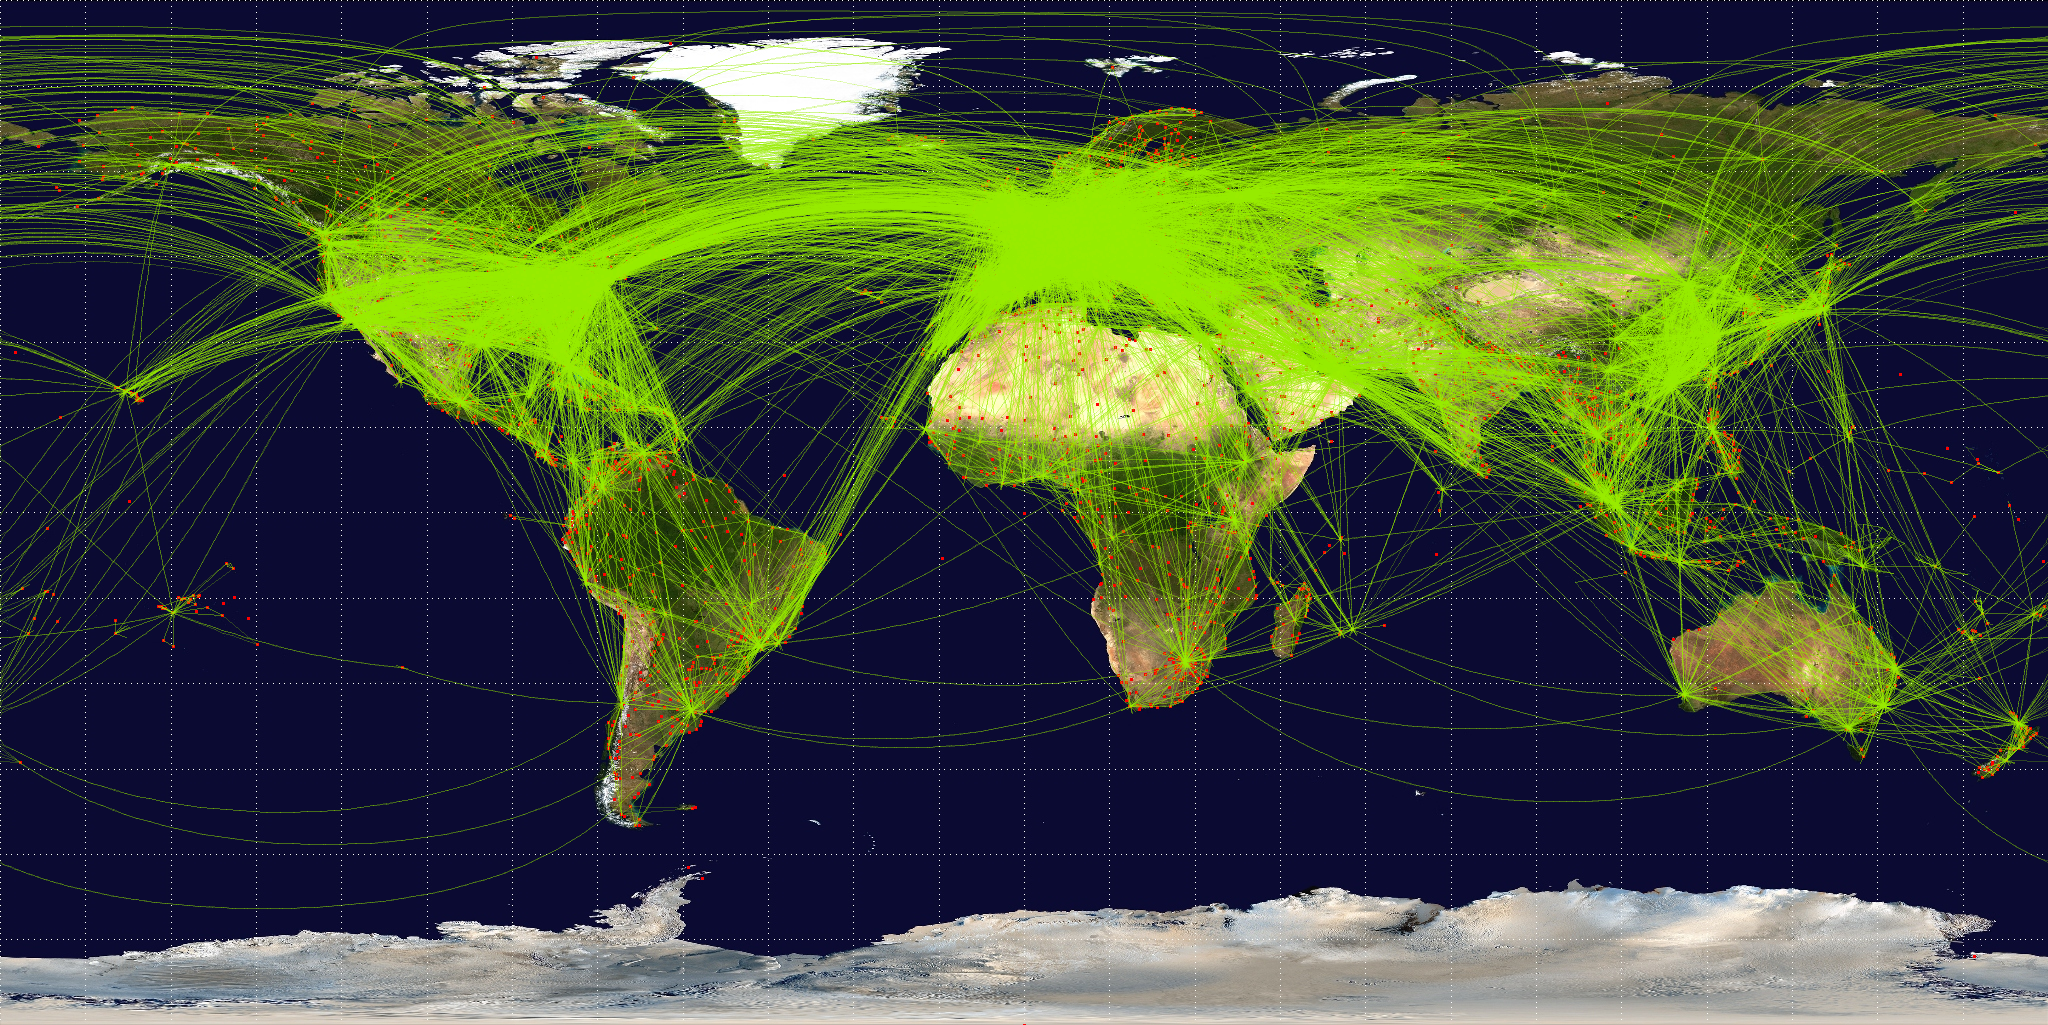
\includegraphics[width=14cm]{images/openflights-routedb} \par
		\vfill \par	\vfill
		\vspace{16mm}
		{\normalsize	سیدمحمدحسین هاشمی  4022363143 \par}
		
		{\normalsize	سیدحسین حسینی  4012363238 \par}
		\vspace{1cm}
		{\large آبان ۱۴۰۲\par}
	\end{titlepage}
	\tableofcontents
	\newpage
	
	
	\section{پکیج های استفاده شده}
	
		{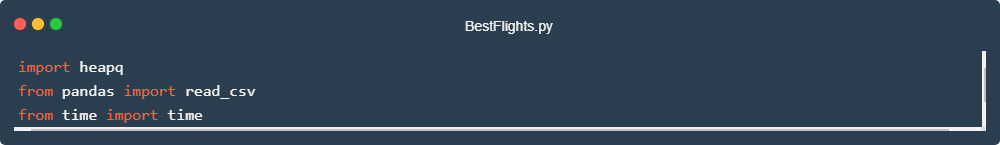
\includegraphics[width=14cm]{images/libraries}}
			
		\begin{itemize}
				
			\item 
				{\Large \lr{heapq}:}
				{\small در تابع \lr{ShortestPath} از این پکیج استفاده شده است.}
				
			\item 
				{\Large \lr{pandas}:}
				{\small برای ایجاد \lr{dataframe} .و تقسیم بندی داده ها مورد استفاده قرار می‌گیرد}
				
			\item 
				{\Large \lr{time}:}
				{\small برای محاسبه زمان اجرای الگوریتم}

		\end{itemize}
			
			
	\section{آماده سازی برای شروع}

		{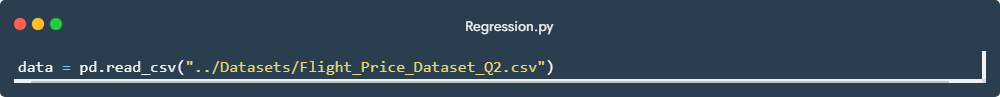
\includegraphics[width=14cm]{images/code01}} \par
		{\normalsize گرفتن ورودی، ‌ساخت دیتافریم و ذخیره زمان شروع اجراالگوریتم}
			
			
	\section{محاسبه وزن الگوریتم}
		
		\subsection{ضرایب} \label{weitghs}
				
			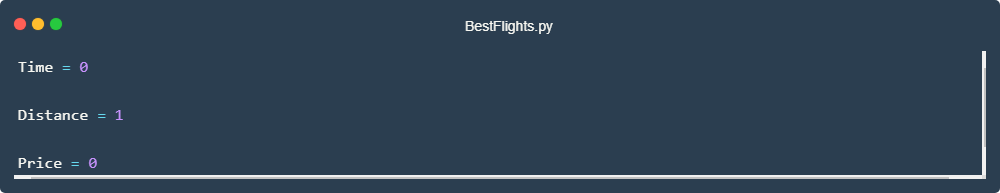
\includegraphics[width=14cm]{images/code02} \par
			{\normalsize سه مقدار: زمان،‌ مسافت و هزینه معیار های قابل امتیاز دهی در بین  داده‌هاست که در این قسمت ضریب هرکدام دریافت و از این مقدار ها در \ref{calculate_func} استفاده خواهد شد.}
				
		\subsection{محاسبه} \label{calculate_func}
				
			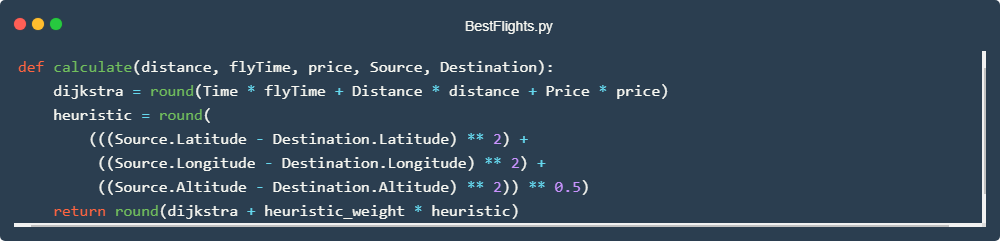
\includegraphics[width=14cm]{images/code03} \par
			{\normalsize با استفاده از ضرایب دریافتی از \ref{weitghs} وزن مسیرها را محاسبه و برمی‌گردانیم.این تابع در کلاس \lr{Eِdge} استفاده می‌شود.}
		
	
	\section{کلاس \lr{Node}} \label{node_class}
	
		{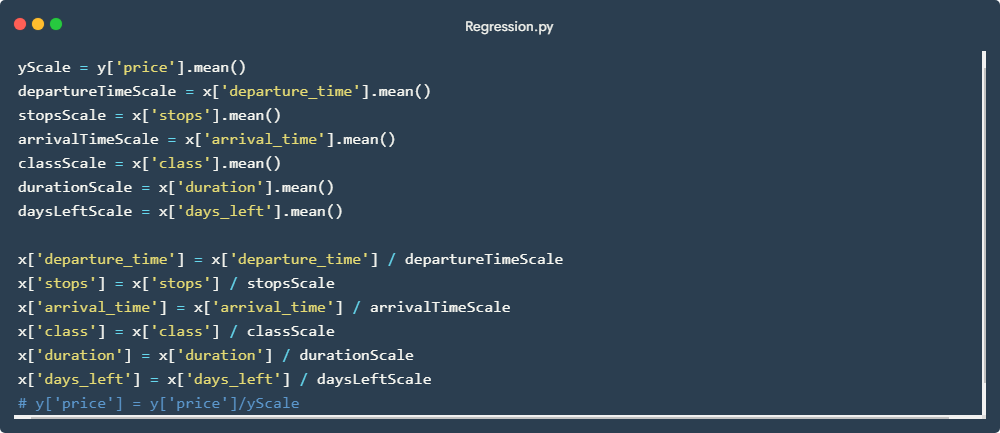
\includegraphics[width=14cm]{images/code04}} \par
		{\normalsize این کلاس برای ذخیره هر گره (فرودگاه)استفاده می‌شود. مقادیر \lr{Airport}،‌ \lr{Airport-Country} و \lr{Ariport-City} را دریافت و ذخیره می‌کند و همچنین از متد \lr{--str--} برای ایجاد خروجی استفاده می‌شود.}
		
		
	\section{کلاس \lr{Edge}} \label{edge_class}
		
		{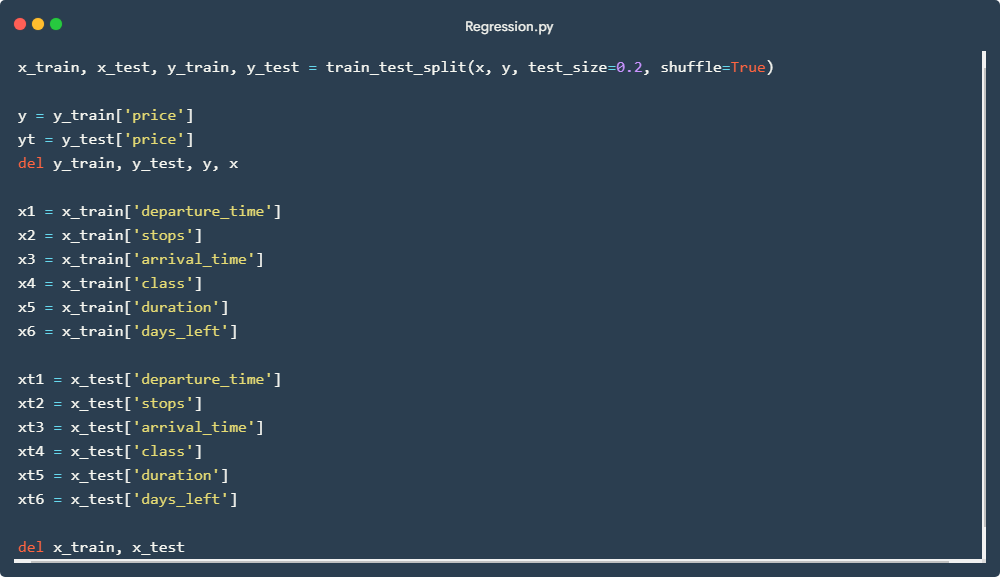
\includegraphics[width=14cm]{images/code05}} \par
		{\normalsize از این کلاس برای ذخیره یک پرواز (مسیر) استفاده می‌کنیم. این کلاس موقع ایجاد کلاس‌های مبدا و مقصد و ویژگی‌های هر پرواز شامل قیمت، مدت پرواز و مسافت را می‌گیرد.
		تابع \lr{calculate} در این قسمت استفاده می‌شود تا وزن مسیر را حساب کند. \par
		متد \lr{--str--} خروجی نهایی هر پرواز را تولید می‌کند و متد \lr{--gt--} برای استفاده در تابع \lr{ShortestPath} ایجاد شده و برای مرتب سازی مسیر ها بر اساس کمترین وزن استفاده می‌شود.}
	
	
	\section{لیست یکتا فرودگاه‌ها} \label{unique_nodes}
	
		{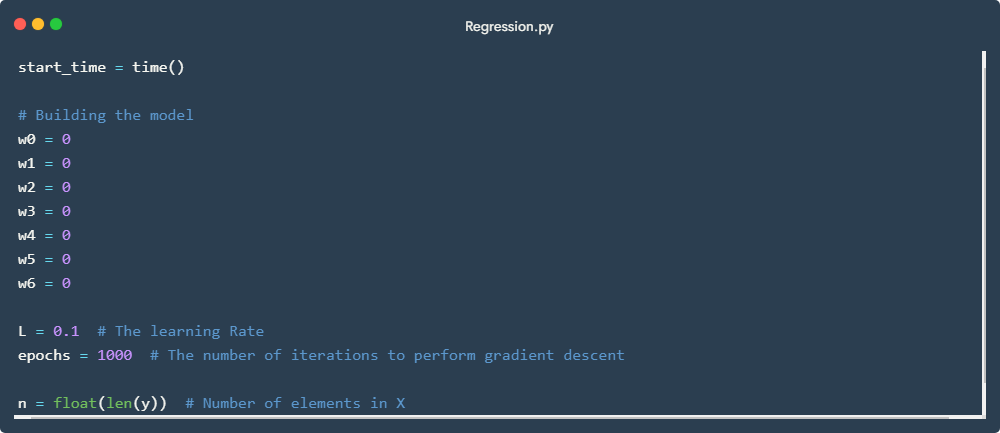
\includegraphics[width=14cm]{images/code06}} \par
		{\normalsize در این قسمت از پروژه فرودگاه‌ها را به صورت یکتا \lr{(Unique)} ذخیره می‌کنیم.
	(این قسمت برای ایجاد لیستی از کلاس های \lr{Node}) ضروری است.}
	
		
	
	\section{لیست کلاس فرودگاه‌ها \lr{(Node class)}} \label{node_list}
	
		{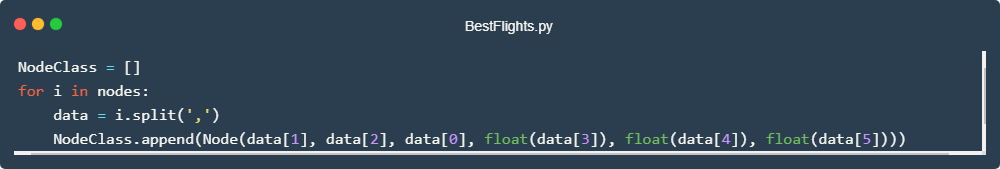
\includegraphics[width=14cm]{images/code07}} \par
		{\normalsize با استفاده از قسمت \ref{unique_nodes} لیستی از کلاس‌های \lr{Node} می‌سازیم که برای پردازش خروجی مورد استفاده قرار می‌گیرد.}
	
	


	\section{لیست پروازها} \label{edges_list}

		{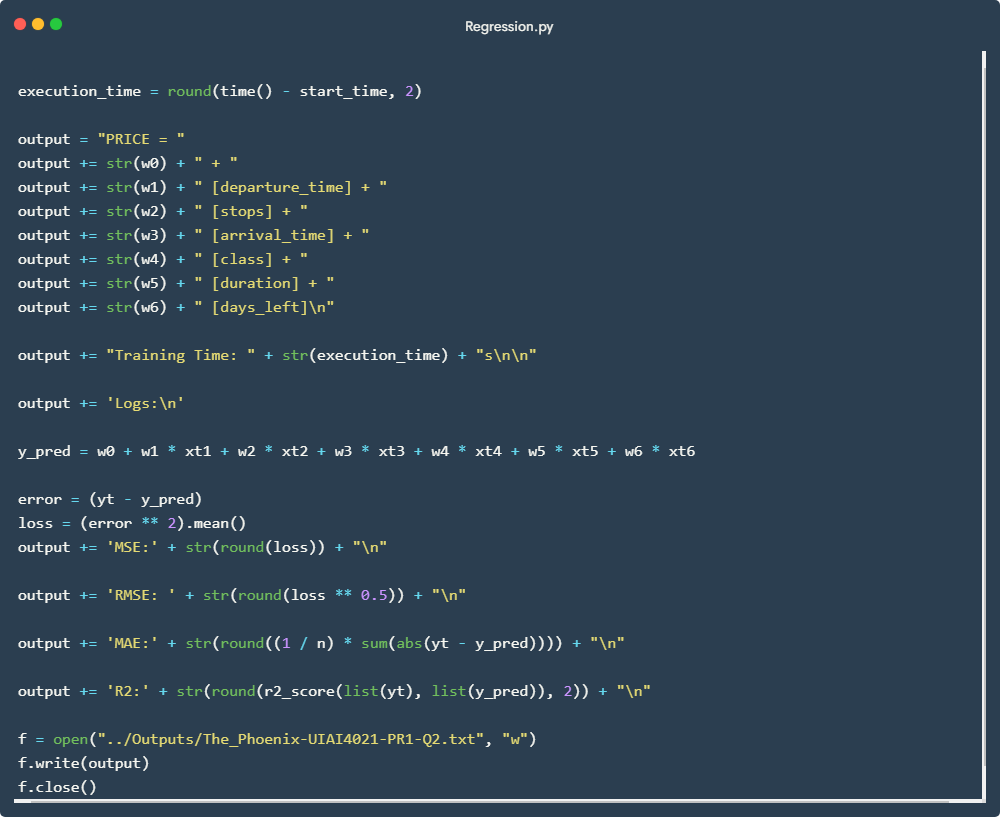
\includegraphics[width=14cm]{images/code08}} \par
		{\normalsize با استفاده از \ref{unique_nodes} و \ref{node_list} لیستی از مسیر ها می‌سازیم که از مقادیر مقصد (\lr{nodes index})، مبدا (\lr{nodes index}) و کلاس قسمت \ref{edge_class} تشکیل می‌شود. این لیست ورودی تابع \ref{calculate_func} می‌باشد.}

	


	\section{محاسبه بهترین مسیر} \label{shortest_path_func}

		{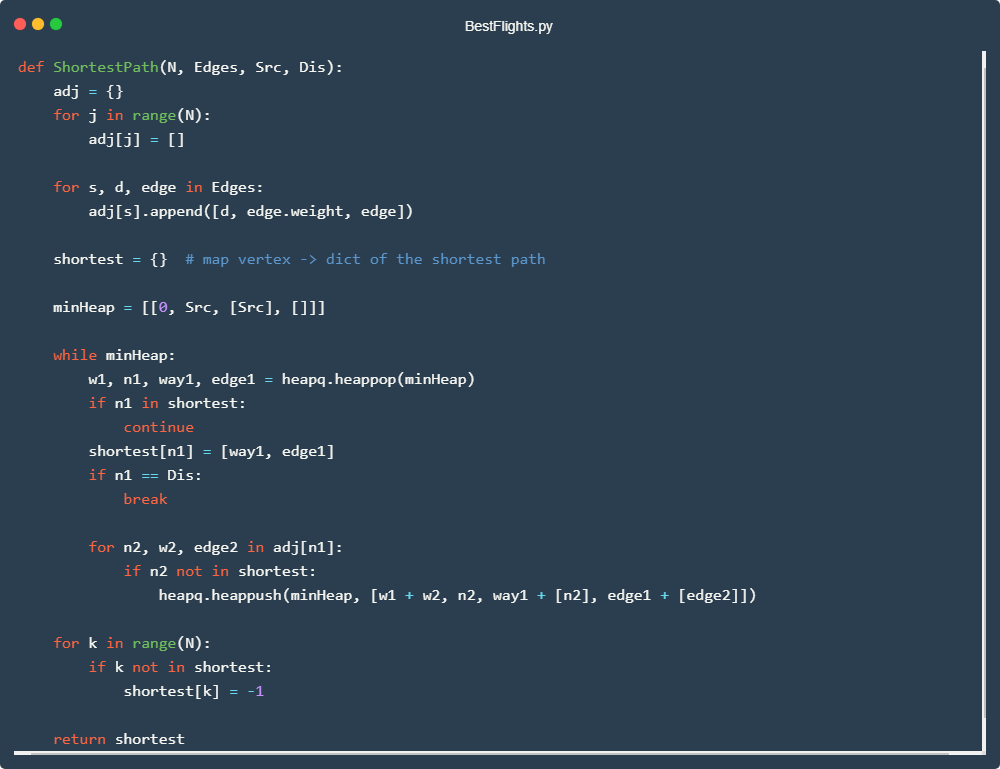
\includegraphics[width=14cm]{images/code09}} \par
		{\normalsize 
		ورودی این تابع به ترتیب تعداد فرودگاه‌ها، لیست مسیرها \ref{edges_list}، شماره گره مبدا و مقصد در لیست \ref{node_list} می‌باشد.
		
		ابتدا یک دیکشنری که در آن به ازای هر فرودگاه یک لیست خالیست می‌سازد و سپس مقادیر آن لیست ها را با مسیرهایی که از آن گره خارج می‌شود پرمی‌کند (هر عنصر افزوده شده به صورت  [کلاس گره \ref{edge_class}، وزن گره و مقصد گره]).
		
		دیکشنری \lr{shortest} برای ذخیره کردن بهترین مسیر هر فرودگاه ایجاد و در ادامه پر می‌شود.
		یک \lr{minHeap} می‌سازیم که مسیرها را د رآن ریخته و هربار کم وزن ترین مسیر را انتخاب کنیم. عناصر درون آن به صورت [مسیر (شامل کلاس های \ref{edge_class})، فرودگاه ها (شامل کلاس های \ref{node_class})، شماره مبدا و مقصد در لیست \ref{node_list}] می‌باشد.
		
		پس از آن با استفاده از حلقه \lr{while} تمامی گره ها را تا قبل از رسیدن به مقصد بررسی می‌کنیم و هربار که به گره جدیدی برسیم آن را در \lr{shortest} ذخیره می‌کنیم و هر بار به گره می‌رسیم مسیرهای خارج شده از آن را به \lr{minHeap} اضافه می‌کنیم.
		}


	\section{پردازش ورودی} \label{input_proccess}

		{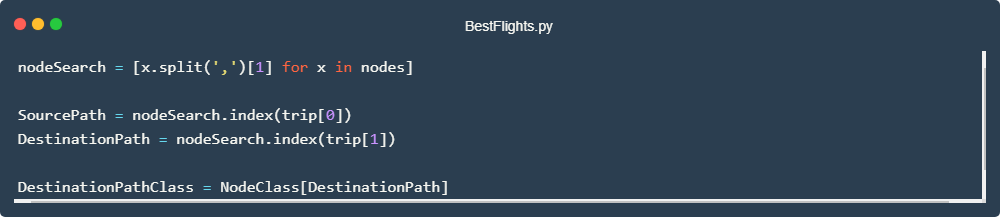
\includegraphics[width=14cm]{images/code10}} \par
		{\normalsize در این قسمت ورودی‌ها را تبدیل به شماره آن‌ها در لیست \ref{node_list} می‌کنیم.}




	\section{جواب های مسئله} \label{answer_ready}

		{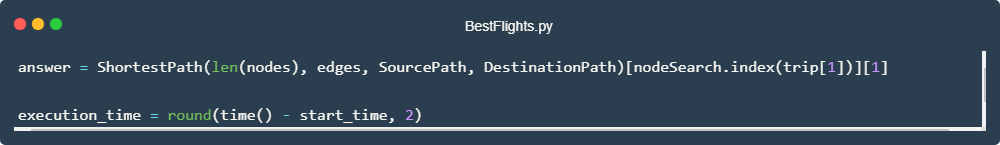
\includegraphics[width=14cm]{images/code11}} \par
		{\normalsize 
		\lr{answer} همان جواب و \lr{execution-time} زمان اجرای الگوریتم است.
		}




	\section{خروجی مسئله} \label{output}

		{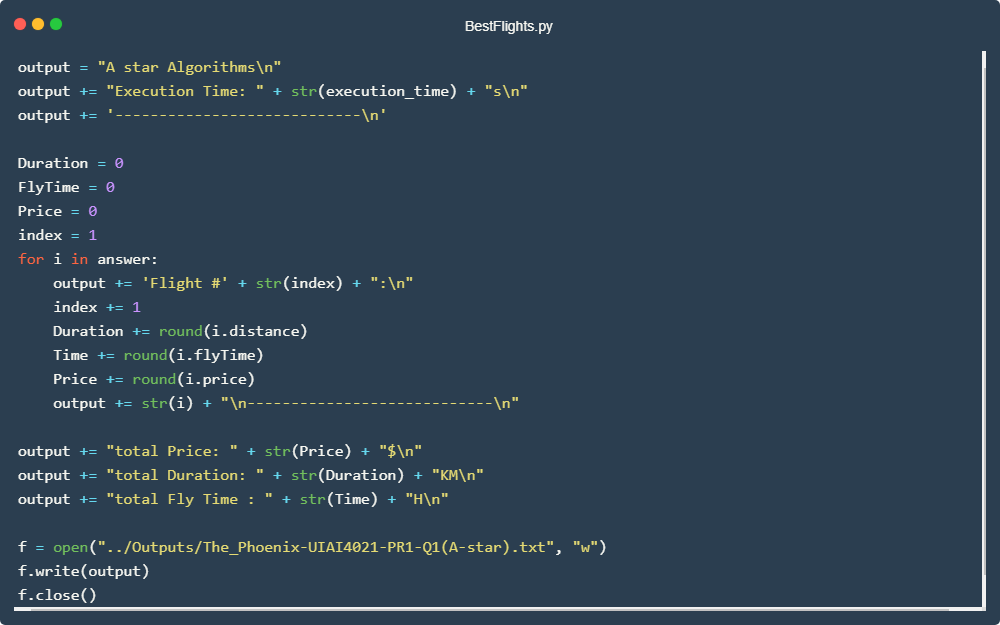
\includegraphics[width=14cm]{images/code12}} \par
		{\normalsize 
		در این قسمت خروجی به فرم خواسته شده اماده و درون فایل با نام خواسته شده ریخته می‌شود.
		}






	\section{منبع} \label{resource}
	
		\begin{itemize}
			
			\item 
			\textbf{\lr{https://youtu.be/XEb7\_z5dG3c?si=hE5rwWGypR5ytY7\_}}

			
		\end{itemize}

		
	
\end{document}